\documentclass[tikz,border=10pt]{standalone}
\usepackage{tikz}
\usetikzlibrary{shapes,patterns,positioning}
\usetikzlibrary{angles, quotes, positioning, arrows.meta, decorations.markings}
\begin{document}
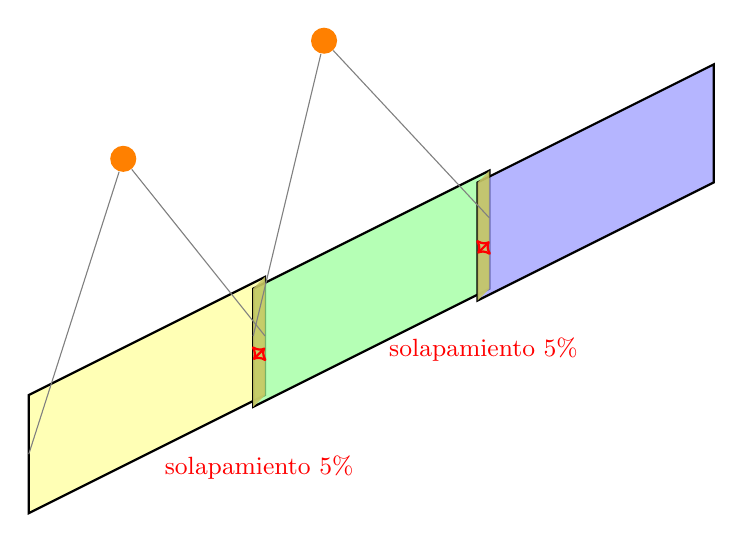
\begin{tikzpicture}[scale=1.5]
    % Definir colores para diferentes swaths
    \definecolor{swath1}{RGB}{255,255,150}  % Amarillo claro
    \definecolor{swath2}{RGB}{150,255,150}  % Verde claro
    \definecolor{swath3}{RGB}{150,150,255}  % Azul claro
    \definecolor{overlap}{RGB}{200,200,100} % Color de solapamiento


    % Primer swath
    \fill[swath1, opacity=0.7] (0,0.5) -- (2,1.5) -- (2,2.5) -- (0,1.5) -- cycle;
    \draw[thick] (0,0.5) -- (2,1.5) -- (2,2.5) -- (0,1.5) -- cycle;

    % Segundo swath con 5% de solapamiento
    \fill[swath2, opacity=0.7] (1.9,1.4) -- (3.9,2.4) -- (3.9,3.4) -- (1.9,2.4) -- cycle;
    \draw[thick] (1.9,1.4) -- (3.9,2.4) -- (3.9,3.4) -- (1.9,2.4) -- cycle;

    % Tercer swath con 5% de solapamiento
    \fill[swath3, opacity=0.7] (3.8,2.3) -- (5.8,3.3) -- (5.8,4.3) -- (3.8,3.3) -- cycle;
    \draw[thick] (3.8,2.3) -- (5.8,3.3) -- (5.8,4.3) -- (3.8,3.3) -- cycle;

    % Marcar zonas de solapamiento
    \fill[overlap, opacity=0.9] (1.9,1.4) -- (2,1.5) -- (2,2.5) -- (1.9,2.4) -- cycle;
    \fill[overlap, opacity=0.9] (3.8,2.3) -- (3.9,2.4) -- (3.9,3.4) -- (3.8,3.3) -- cycle;

    % Satélites en órbitas
    \node[circle, fill=orange, minimum size=8pt] (sat1) at (0.8,3.5) {};
    \node[circle, fill=orange, minimum size=8pt] (sat2) at (2.5,4.5) {};


    % Líneas de vista desde satélites
    \draw[thin, gray] (sat1) -- (0,1);
    \draw[thin, gray] (sat1) -- (2,2);
    \draw[thin, gray] (sat2) -- (1.9,2);
    \draw[thin, gray] (sat2) -- (3.9,3);

    % Indicar porcentaje de solapamiento
    \draw[<->, red, thick] (1.9,1.8) -- (2,1.9);
    \node[red, above] at (1.95,0.7) {\small solapamiento 5\%};

    \draw[<->, red, thick] (3.8,2.7) -- (3.9,2.8);
    \node[red, above] at (3.85,1.7) {\small solapamiento 5\%};

\end{tikzpicture}

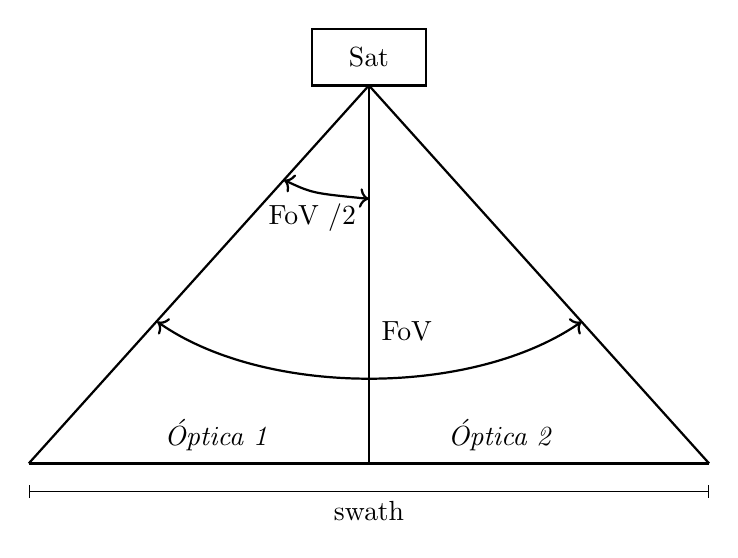
\begin{tikzpicture}[scale=1.2]

% Satélite
\draw[thick] (0,4) rectangle (1.2,4.6);
\node at (0.6,4.3) {Sat};

% Línea central
\draw[thick] (0.6,4) -- (0.6,0);

% Pirámide de visión
\draw[thick] (0.6,4) -- (-3,0);
\draw[thick] (0.6,4) -- (4.2,0);

% Línea base (swath)
\draw[thick] (-3,0) -- (4.2,0);

% Etiqueta de swath
\draw[|-|] (-3,-0.3) -- (4.2,-0.3);
\node at (0.6,-0.5) {swath};

% Ángulo FoV
\draw[<->,thick] (-0.3,3) .. controls (-0,2.86)  .. (0.6,2.8);
\node at (-0.0,2.6) {FoV /2};

% Ángulo FoVx2
\draw[<->,thick] (-1.64,1.5) .. controls (-0.5,0.7) and (1.7,0.7) .. (2.85,1.5);
\node at (1,1.4) {FoV};

% Etiquetas adicionales
\node at (2.5,2) { };
\node at (-1.0,0.3) {\textit{Óptica 1}};
\node at (2.0,0.3) {\textit{Óptica 2}};
\end{tikzpicture}


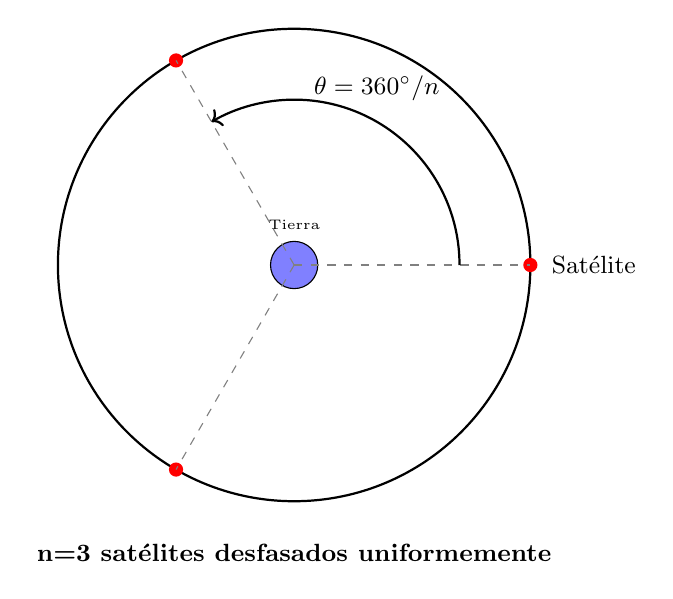
\begin{tikzpicture}[scale=3]

% Dibuja la órbita
\draw[thick] (0,0) circle (1);

% Dibuja la Tierra
\filldraw[fill=blue!50] (0,0) circle (0.1);
\node at (0,0.17) {\tiny Tierra};

% Satélites (n=3) y líneas angulares
\foreach \i in {0,1,2} {
    % Posición del satélite
    \coordinate (S\i) at ({cos(120*\i)},{sin(120*\i)});
    % Satélite como punto rojo
    \fill[red] (S\i) circle (0.03);
    % Línea discontinua del centro al satélite
    \draw[dashed,gray] (0,0) -- (S\i);
}

% Arco para indicar el ángulo theta
\draw[->,thick] (0.7,0) arc (0:120:0.7);
\node at ({0.7*cos(60)},{0.7*sin(60)+0.14}) {\small $\theta = 360^\circ/n$};

% Texto explicativo
\node at (0,-1.22) {\small \textbf{n=3 satélites desfasados uniformemente}};

% Leyenda en recuadro


    \node[right] at (1.05,0) {\small Satélite};


\end{tikzpicture}

\end{document}
